% !TEX root = ../thesis.tex
% adjust number of reference angles
% @author Tobias Wulf
%

\section{Anpassung der Referenzwinkelanzahl}\label{sec:exp2}


\textbf{Zweck:} Das Experiment soll einen Bereich abstecken für die Wahl der Anzahl für gleichverteilte Referenzwinkel. Dafür wird die äußere Modelloptimierung über das Rauschniveau nach \autoref{alg:bayesopt} ausgeschaltet und ein konstantes Rauschniveau $\sigma_n^2$ vorgeben. Das Regressionsmodell wird daher nur für die Längen- und Höhenskalierung $\theta = (\sigma_f^2, \sigma_l)$ der Kovarianzfunktion optimiert, siehe \autoref{alg:fminconopt}. Verglichen wird das Regressionsmodell für euklidischen Abstand nach \autoref{eq:de2innorm} und \autoref{eq:kfun} einmal ohne unterstützende Mittelwertbildung über Polynome (Zero-Mean) und mit Polynombildung ersten Grades, siehe \autoref{eq:hfun} bis \autoref{eq:gprmean}. Diese wirkt als eine Offset- und Amplitudenkorrektur der Messwerten. Es werden absolute mittlere und maximale Winkelfehler in Abhängigkeit der Referenzwinkelanzahl verglichen. Zusätzliche wird die Berechnungsdauer einer Winkelvorhersage in Abhängigkeit der Referenzwinkelanzahl bzw. Trainingspunkte aufgenommen. Im besten Fall stellt sich heraus, dass das Mittelwert freie Verfahren gleich oder besser ist gegenüber dem Polynom gestützten Verfahren. Die Umsetzung des letzteren Verfahrens ist deutlich aufwendiger zu gestalten und birgt einige numerischer Fehleranfälligkeiten und Hürden, die es in den Griff zu bekommen gilt.

\textbf{Durchführung:} Es werden zwei Modelle mit euklidischer Abstandfunktion initialisiert und Trainiert, jeweils mit und ohne unterstützendes Mittelwertpolynom. Jedes der beiden Modelle wird mit pro Durchgang mit gleichem Trainingsdaten trainiert und anschließend die Skalierung der Kovarianzfunktion in Länge und Höhe entsprechend der Trainingsdaten getrimmt. Danach wird die Zeit gemessen, die es benötigt einen Simulationswinkel zu vorherzusagen. Jeweils getrennt für beide Modelle. Zum Ende des Durchgangs werden absolute Winkelfehler auf eine volle Rotation mit einem Testdatensatz über $720$ Winkeln bei einer Auflösung von $\SI{0,5}{\degree}$ berechnet und für mittlere sowie maximale Winkelfehler über die gesamte Rotation ausgewertet. Ebenfalls für beide Modelle. Der Durchgang wird für jeden zur Verfügung stehenden Trainingsdatensatz wiederholt. Der Testdatensatz bleibt für jeden Durchgang gleich. Alle Datensätze sind für die gleiche Position des Sensors und bei gleicher Verkippung des Magneten zuvor prozessiert worden.

\textbf{Erzeugte Datensätze:} Es sind für das Experiment 12 Trainingsdatensätze mit unterschiedlicher Referenzwinkelanzahl und ein Testdatensatz erzeugt worden. Alle Datensätze korrespondieren in Position und Verkippung.

\textbf{Matlab-Skript:} compareCpuTimeVsError.m, siehe \autoref{mcode:comparecputimevserror}.


\clearpage


\textbf{Abweichende Parameter von \autoref{tab:sim-params-exp}:}

\begin{itemize}
	\item TrainingsOptions: nAngles: $\left\{ 8, 16, 24, 32, 40, 48, 60, 80, 120, 240, 360, 720 \right\}$
	\item GRPOptions: kernel : 'QFCAPX'
	\item GPROptions: mean: 
	\begin{itemize}
		\item[a.] 'zero'
		\item[b.] 'poly'
	\end{itemize}
\end{itemize}

\textbf{Ergebnisse:} Die Ergebnisse des Experiments sind grafisch in \autoref{fig:timings-vs-errors} ausgewertet. Berechnungszeiten für einen Simulationswinkel a) sowie mittlerer b) und maximaler c) absoluter Winkelfehler bei voller Rotation sind in Abhängigkeit der Referenzwinkelanzahl in den Trainingsdatensätzen aufgetragen.

\textbf{Beobachtungen:} Die Messung der Berechnungszeit für eine Simulationswinkelvorhersage in a) ergibt, dass beide Implementierungskonfigurationen annähernd gleich schnell sind und die Rechenzeit bis eine Referenzwinkelanzahl von $N_{Ref} = 80$ mit leichten Abweichungen konstant bleibt. Für eine Referenzwinkelanzahl von $N_{Ref} > 80$ nimmt die Rechenzeit für beide Varianten gleichermaßen exponentiell zu. Für absolute mittlere und maximale Winkelfehler unterscheiden sich die mittelwertfreie und Polynom gestützte Variante nur bei $N_{ref} = 8$. Dort liefert jeweils die mittelwertfreie Variante den geringeren Winkelfehler. Für eine Referenzwinkelanzahl $N_{Ref} > 8$ liefern beide Variationen einen annähernd gleichen Winkelfehler. Bei einer Referenzwinkelanzahl von $N_{Ref} = 48$ gibt es eine Sprungstelle für den mittleren und maximalen Winkelfehler, beide mittlerer sowie maximaler Winkelfehler verringern sich ungefähr um die Hälfte. Der Winkelfehler bleibt nach dem Sprung konstant und schwankt nur noch minimal. Dieser Bereich (2) ist in den Abbildungen b) und c) grau unterlegt und weißt im Vergleich zu Bereich (1) weniger Fehlerdynamik für nachfolgende Optimierungsschritte auf. Der interessante Bereich (1) für eine weitere Optimierung über das Rauschniveau $\sigma_n^2$ nach \autoref{alg:bayesopt} ist in a), b) und c) grün unterlegt. Diesen gilt es im weiteren Verlauf anzupassen und die Sprungstelle in b) und c) zu verkleinern oder auszulöschen.


\clearpage
\begin{landscape}
\begin{figure}[tbph]
	\centering
	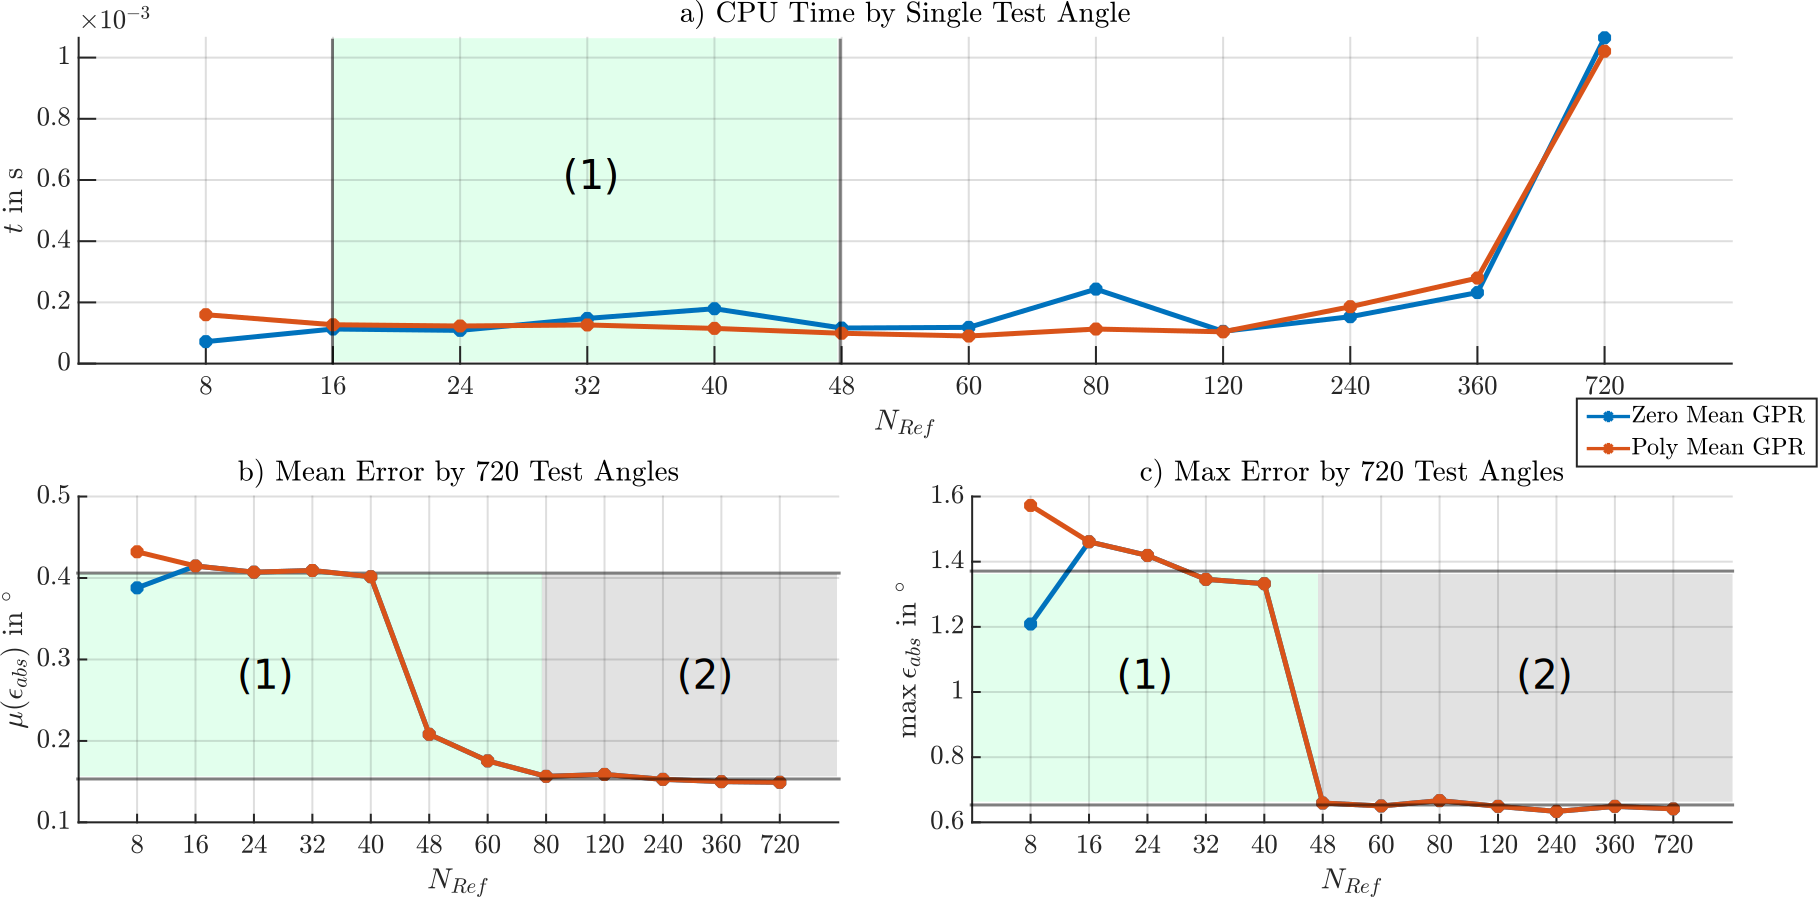
\includegraphics[width=\linewidth]{chapters/images/4-EuOExp/Timings-vs-Errors}
	\caption[Variation der Referenzwinkelanzahl bei konstantem Rauschniveau]{Variation der Referenzwinkelanzahl bei konstantem Rauschniveau $\sigma_n^2 = 10^{-6}$. Es wird die Implementierung des Regressionsmodell nach \autoref{eq:kfun} mit euklidischen Abstand nach \autoref{eq:de2innorm}, jeweils ohne (Zero Mean GPR) und mit Mittelwertunterstützung (Poly Mean GPR) in Abhängigkeit der Referenzwinkelanzahl $N_{Ref}$ verglichen. Dafür wird in a) die Berechnungszeit eines Simulationswinkel gemessen und in b) der absolute mittlere Winkelfehler, sowie in c) der absolute maximale Winkelfehler auf eine volle Rotation ausgewertet. Die jeweiligen initiierten Modellvariation sind für ihre Kovarianzfunktionsparameter $\theta = (\sigma_f^2,\sigma_l)$ getrimmt nach \autoref{alg:fminconopt}. Die Optimierung des Rauschniveaus $\sigma_n^2$ nach \autoref{alg:bayesopt} ist ausgeschaltet. Modelltrainingsdaten basieren hier für beide Varianten auf Vektoren bzw. Skalare.}
	\label{fig:timings-vs-errors}
\end{figure}
\end{landscape}


\clearpage

